\chapter{Setting up a Markov Model}
While our simulations provide empirical insights into game duration, a Markov Chain model allows for analytical predictions of expected game length and transient state probabilities.
In this chapter, an analytical framework based on Markov chain theory to model the dynamics of Snakes and Ladders is utilised. This approach provides a rigorous method for quantifying game progression and predicting key metrics, such as the expected number of turns to reach the final board position. 

\section{What are Markov Chains}
A Markov chain is a mathematical system that experiences transitions from one state to another in a chain-like process. Its defining characteristic is the memoryless property: the probability of transitioning to the next state depends solely on the current state and not on the sequence of events that preceded it. In the context of Snakes and Ladders, each board position is treated as a state, and the outcome of a dice roll determines the probability of moving from one state to another.

By adopting a Markov chain framework, the random nature of the game can be captured, where each dice roll is independent—and incorporate the special rules governing snakes and ladders. This model enables a transition beyond empirical simulation and derive analytical expressions for key performance measures, such as the average number of moves required to complete the game.

\section{Fundamental Concepts}
Before detailing the construction of our model, it is important to define several key concepts:
\begin{enumerate}
	\item 	\textbf{States:} In our model, each tile on the board (from 0 to the board size) represents a state. The starting position is state 0, and the final position (the goal) is an absorbing state, meaning that once reached, no further transitions occur.
	\item \textbf{Transitions:} A transition is the movement from one state to another. In Snakes and Ladders, transitions occur as a result of dice rolls. Each roll yields one of six outcomes (with equal probability of 	$\frac{1}{6}$), which, when added to the current position, determine the next state.
	\item \textbf{Absorbing States: }An absorbing state is one that, once entered, cannot be left. In our game, the final tile is an absorbing state because the game terminates when the player reaches or exceeds it.
	\item \textbf{Memorylessness: }The Markov property implies that the probability of moving to a new state depends solely on the current state, not on how that state was reached. This simplifies the analysis, as the past history of the game does not need to be considered when determining future moves.
\end{enumerate}

\section{Constructing the Transition Matrix}
The transition matrix is a square matrix $P$ of dimensions $(N- (N_S+N_L))  \times (N- (N_S+N_L))$ (where $N$ is the board size), and each entry $P(i,j)$ represents the probability of moving from state $i$ to state $j$ in one turn. $N_S$ and $N_L = 10$ and their lengths are randomly assigned using the fixed start and end points approach from Chapter 2.

\subsection{Methodology}
For each non-absorbing state (i.e. every state except tile 100):
\begin{enumerate}
	\item \textbf{Dice Roll Outcomes:} The agent rolls a fair six-sided die. Each outcome, $k$ (where $1 \leq k \leq 6$), occurs with probability $\frac{1}{6}$
	\item \textbf{Movement Calculation:} The tentative new state is calculated by adding the dice roll $k$ to the current state $i$. If the tentative new state exceeds the board limits, the excess is subtracted from the final state. This ensures that the player remains on a valid tile.
	\item \textbf{Entity Adjustments:} If the resulting state corresponds to the head of a snake or the base of a ladder, the state is immediately updated to the corresponding tail or top, respectively. 
	\item \textbf{Matrix Population:} For each dice outcome, the appropriate transition probability is added to the matrix entry corresponding to the final state after making all adjustments
\end{enumerate}

For the absorbing state (the final board position), the row in the matrix is set to have a probability of 1 for the remaining in that state, reflecting that no further moves occur once the goal is reached.

For all non-absorbing states $i$:
\[
P(i, j) = \sum_{k=1}^{6} \frac{1}{6} \cdot \mathbf{1}\{\text{if } f(i,k) = j \}
\]
where $f(i,k)$ is the function that computes the new state after adding the dice roll $k$ to state $i$, applying reflection if necessary, and adjusting for any snake or ladder. The indicator function $\mathbf{1}\{\cdot\}$ equals 1 if the condition is met, and 0 otherwise.

\[
P(N, N) = 1 \quad \text{and} \quad P(N, j) = 0 \quad \text{for} \quad j \neq N.
\]

This formulation guarantees that each row of the transition matrix sums to 1, thereby satisfying the properties of a stochastic matrix.

\section{Expected Turns via the Fundamental Matrix}

To determine the average number of moves required to reach the absorbing state from the starting state, the research employs the concept of the \textit{fundamental matrix}.

\subsection{Partitioning the Matrix}

The transition matrix $P$ is partitioned into two segments:
\begin{itemize}
	\item $Q$: The submatrix corresponding to the transient states (all states except the absorbing state).
	\item $R$: The submatrix describing transitions from transient states to the absorbing state.
\end{itemize}

\subsection{Fundamental Matrix Calculation}

The fundamental matrix $N$ is computed as:
\[
N = (I - Q)^{-1}
\]
where $I$ is the identity matrix of the same dimension as $Q$. The entry $N(i, j)$ represents the expected number of times the process is in state $j$ when starting from state $i$ before absorption occurs.

\subsection{Deriving Expected Turns}

The expected number of turns $t$ required to reach the absorbing state from the initial state (state 0) is given by summing the entries in the first row of $N$:
\[
t = \sum_{j} N(0, j)
\]
This sum reflects the total expected visits to all transient states, effectively yielding the average number of turns needed to complete the game.

\section{Findings}
Upon comparing the findings from the Markovian approach with the empirical results obtained through simulations the following was observed:

\subsection{Comparison of Expected Turns}

A primary validation of our Markov model lies in comparing the expected number of turns calculated analytically with the average number of turns observed in simulations. For the specific board configuration (Figure \ref{fig:boardlayout}) generated for this analysis, simulations across 10,000 games yielded an average game duration of \textbf{33.99 turns}.  In stark agreement, the expected number of turns calculated using the fundamental matrix of our Markov model is \textbf{33.72 turns}. This close correspondence (a difference of less than 1\%) strongly supports the validity of our Markov chain model in accurately predicting the average game length for Snakes and Ladders. 

\begin{figure}
	\centering
	\includegraphics[width=0.7\linewidth]{"../Markov Modelling/Data/BoardLayout"}
	\caption{Board Layout used for Simulations and Implementing the Markov Chain}
	\label{fig:boardlayout}
\end{figure}

\subsection{Distribution of Game Turns: Simulation vs. Markov Model}

Beyond the average game time, to further validate the Markov model the distribution of game turns was compared. Figure \ref{fig:frequencydistributionMarkov} displays the probability distribution of game turns obtained from our 10,000 simulations for the chosen board layout alongside the distribution obtained by using the transition probabilities encoded within the transition matrix. This involved starting at state 0, and in each step, probabilistically transitioning to the next state based on the probabilities in the matrix. By repeating this process for a large number of simulated games (again, 10,000 in our analysis), a turn distribution was derived directly from the Markov model.

\begin{figure}[th]
	\centering
	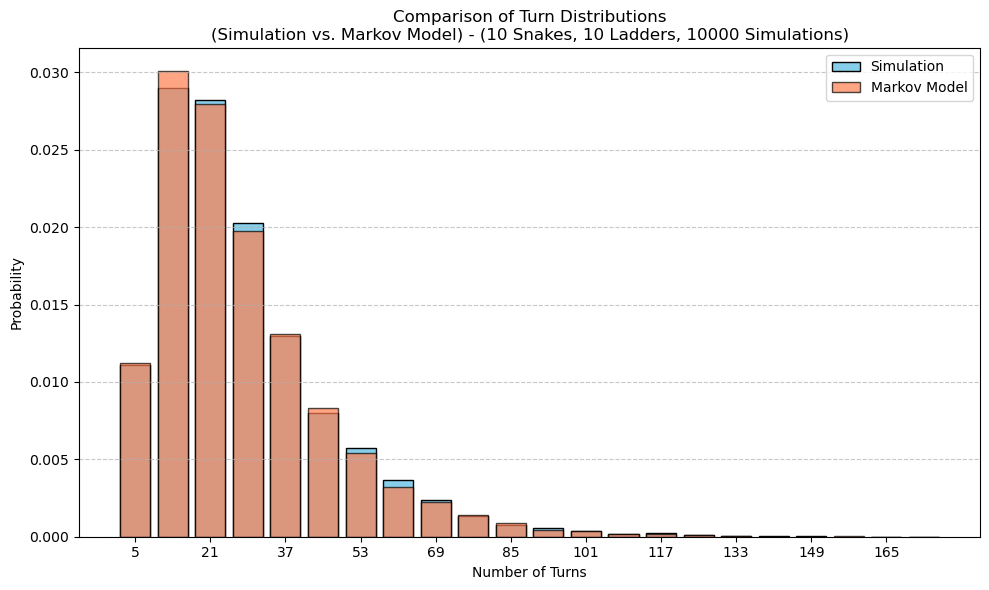
\includegraphics[width=0.7\textwidth]{"../Markov Modelling/Data/FrequencyOveralyed.png"}
	\caption{\textbf{Distribution of Game Turns: Simulation vs. Markov Model (10 Snakes, 10 Ladders, 10,000 Simulations:)} Both distributions seem to overlay each other with an insignificant amount of outliers}
	\label{fig:frequencydistributionMarkov}
\end{figure}

While a direct overlay of the two distributions is visually complex due to the discrete nature of turn counts, a qualitative comparison reveals a strong similarity in their shapes and central tendencies. Both distributions exhibit a right-skewed pattern, with a peak around the 10-20 turn mark and a long tail extending to higher turn counts. The histogram derived from agent-based simulations (as shown in Figure \ref{fig:frequencydistributionMarkov}) closely mirrors the distribution generated from the Markov model's transition probabilities, further reinforcing the model's capacity to capture the stochastic dynamics of game progression.

\subsection{Steady-State Distribution and Hotspot Analysis}

The steady-state distribution, derived analytically from the Markov model, offers insights into the long-term probabilities of occupying each tile on the board. Figure \ref{fig:steady_state_heatmap_chapter3} (b) presents a heatmap visualization of this steady-state distribution. 

\begin{figure}[ht]
	\centering
	\subfloat[]{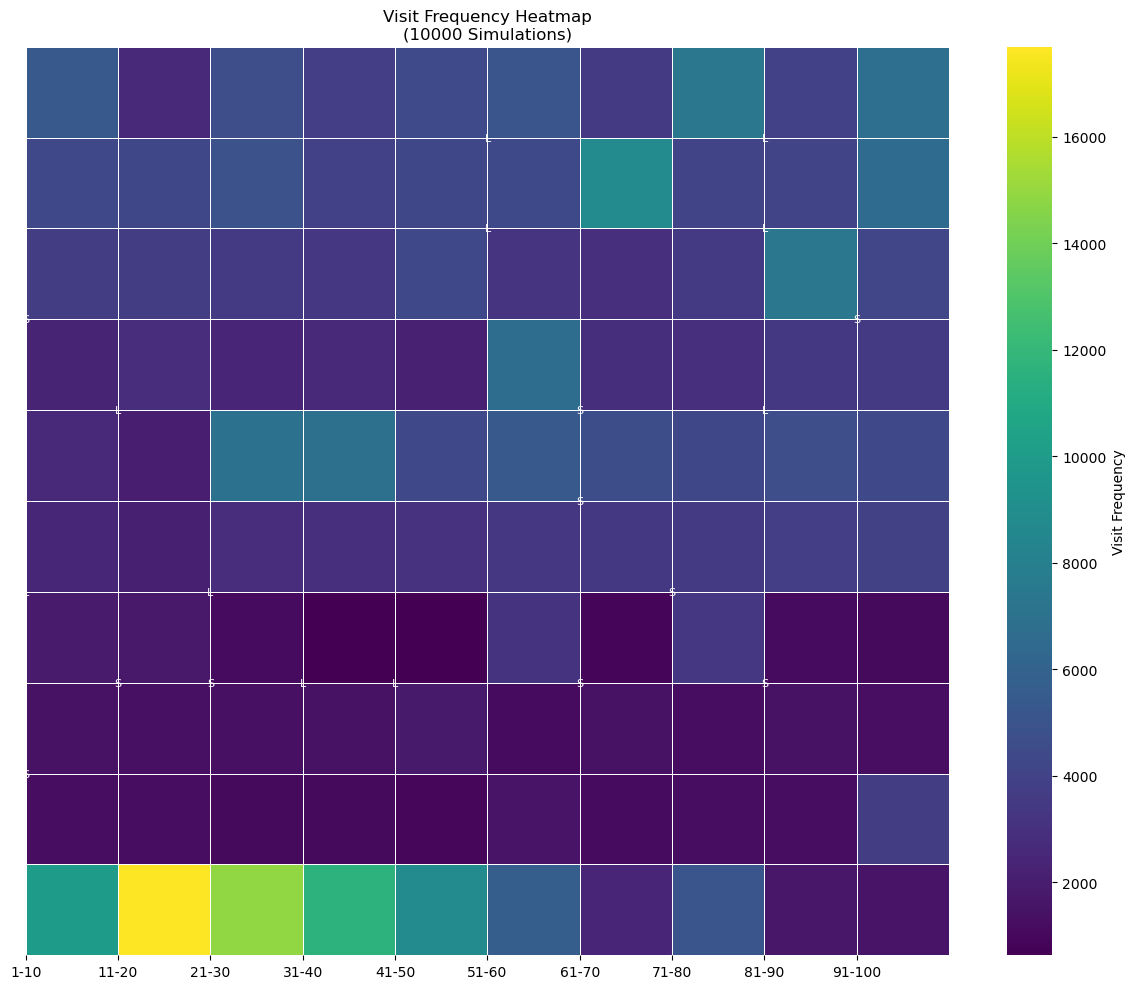
\includegraphics[width=0.45\textwidth]{"../Markov Modelling/Data/TileVisitHeatmap.png"}}
	\subfloat[]{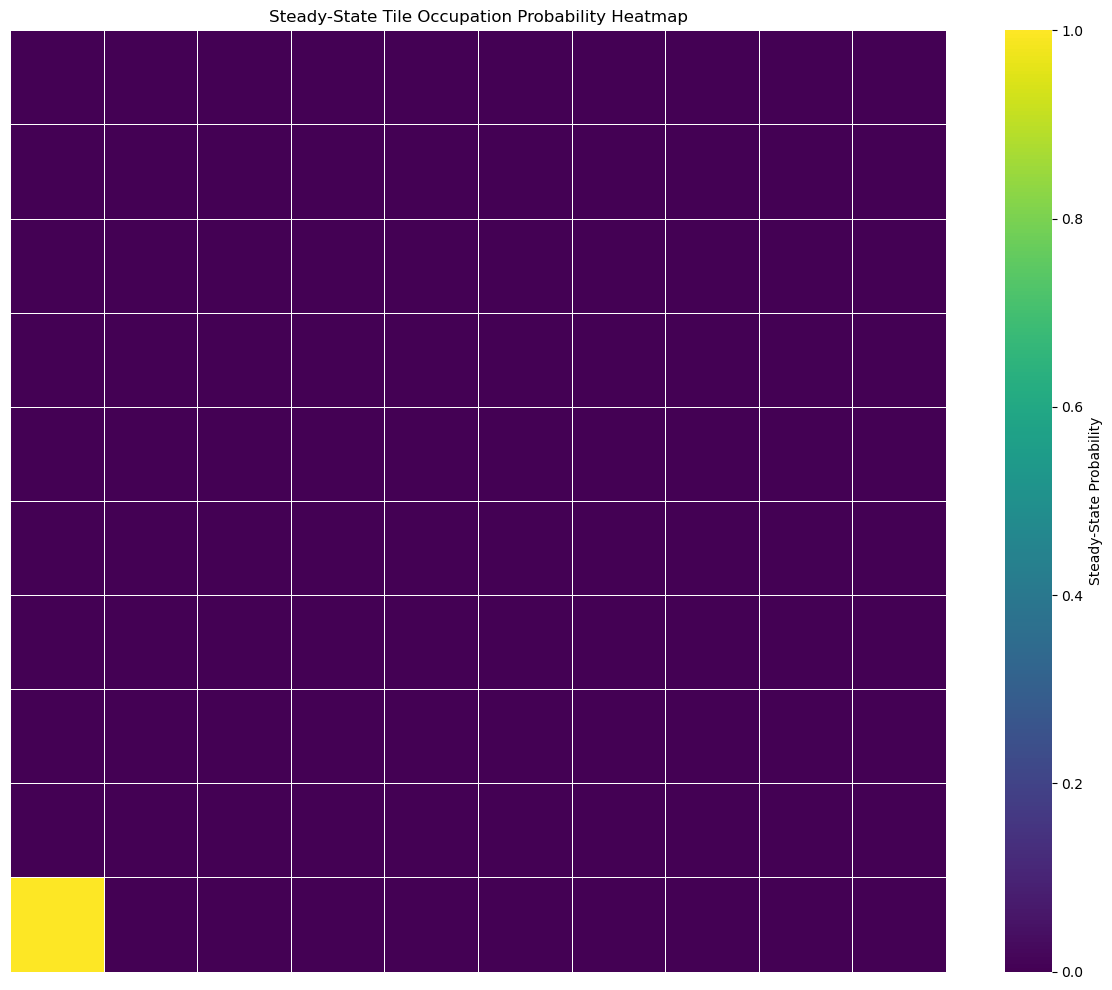
\includegraphics[width=0.45\textwidth]{"../Markov Modelling/Data/SteadyStateHeatmap.png"}}
	\caption{Comparison of Heatmaps: (a) Tile Visit Frequency Heatmap from Agent-Based Simulations, (b) Steady-State Tile Occupation Probability Heatmap from Markov Model}
	\label{fig:steady_state_heatmap_chapter3}
\end{figure}

As expected for a well-formulated absorbing Markov chain, the Steady-State Heatmap (Figure \ref{fig:steady_state_heatmap_chapter3} (b)) shows a probability of 1.0 concentrated on tile 100 (bottom-right corner), with probabilities for all other tiles approaching zero. This indicates that in the long-term, the system predictably ends in the absorbing winning state.

For understanding tile occupation patterns during active gameplay, the Tile Visit Frequency Heatmap from simulations (Figure \ref{fig:steady_state_heatmap_chapter3} (a)) was referred. This heatmap empirically highlights tiles that are landed on most frequently during game progression.  While the Steady-State Heatmap demonstrates the expected long-term behavior of the absorbing Markov chain, it is the Tile Visit Frequency Heatmap that provides insights into gameplay hotspots and relative tile importance during a typical game session.


\subsection{Analytical Derivation of Game Time}

A key advantage of the Markov model is its capacity to analytically derive the expected game time through the fundamental matrix calculation. Unlike simulations, which provide an approximation of the average game time based on repeated trials, the Markov model offers a direct, deterministic calculation of the expected value. This analytical solution, provides a more rigorous and computationally efficient method for determining average game durations for different board configurations and parameter settings. The close agreement between the analytical expected turns and the simulation-based average turns, as highlighted earlier, validates the Markovian approach as a robust and accurate tool for analysing game time in Snakes and Ladders.

\section{Conclusion}

So far, the research successfully leveraged the validated Markov model to conduct a systematic analysis of Snakes and Ladders. By analytically varying the number and lengths of snakes and ladders, the combined impacts have been quantified and a method to formulate the expected game duration has been established. The findings reveal clear trends: increasing snake count and snake lengths generally prolong game time, while increasing ladder count and ladder lengths tend to shorten it.  Additionally, the choice of length distribution significantly influences game pace and variability, with exponential distributions leading to longer, more variable games, and uniform distributions resulting in shorter, more predictable experiences.

Therefore, this chapter paves the way for a more normative investigation into game design, specifically the concept of an ``optimal'' board layout. Having established a method for quantifying how parameters influence game dynamics, the next logical step is to explore what constitutes a desirable or ``optimal'' configuration of snakes and ladders. The next chapter will build upon these findings, shifting from descriptive analysis to a more prescriptive approach. We will explore the notion of board layout optimality, additionally comparing analytically generated ``optimal'' boards with configurations found in commercially available Snakes and Ladders games. This will allow us to assess whether and how real-world game designs implicitly embody or deviate from mechanically ``optimal'' configurations as suggested by our Markovian analysis.
